% diagram_lora_injection.png
% Zoom of one weight matrix: frozen W in parallel with the small trained pair A, B.
% Canvas: 15.23 cm x 3.60 cm (= \textwidth of the deck, height <= 5.0 cm).
\documentclass[border=0pt,11pt]{standalone}
\usepackage[T1]{fontenc}
\usepackage{lmodern}
\renewcommand{\familydefault}{\sfdefault}
\usepackage{amsmath}
\usepackage{tikz}
\usetikzlibrary{positioning,arrows.meta}

\definecolor{primaryNavy}{RGB}{24,24,27}
\definecolor{secondaryNavy}{RGB}{63,63,70}
\definecolor{mutedGray}{RGB}{248,250,252}
\definecolor{ruleGray}{RGB}{226,232,240}

\tikzset{
  box/.style={draw=secondaryNavy, line width=0.6pt, fill=mutedGray, rectangle,
              inner xsep=5pt, inner ysep=2.5pt, align=center,
              text=primaryNavy, font=\small},
  ar/.style={draw=secondaryNavy, line width=0.6pt,
             -{Latex[length=1.4mm,width=1.0mm]}},
  ln/.style={draw=secondaryNavy, line width=0.6pt},
  note/.style={text=primaryNavy, font=\footnotesize, align=center},
}

\begin{document}
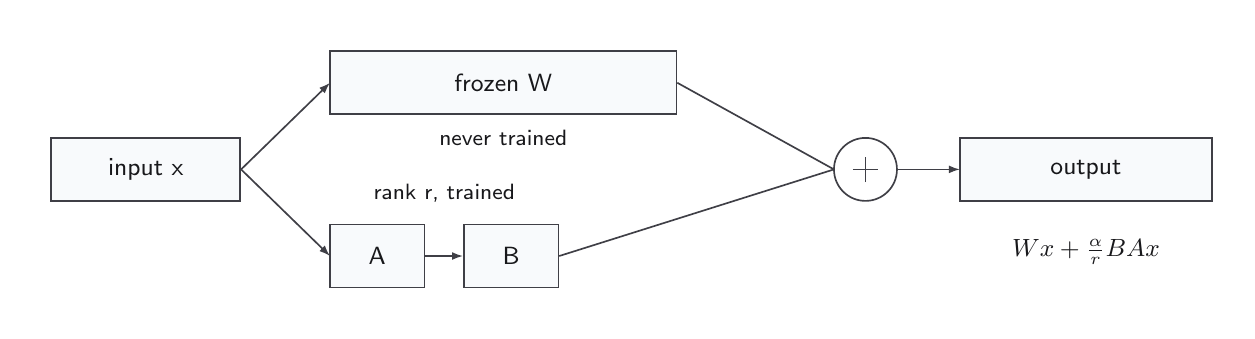
\begin{tikzpicture}[x=1cm,y=1cm]
\useasboundingbox (0,0.80) rectangle (15.23,4.40);
\fill[white] (0,0.80) rectangle (15.23,4.40);

% ---------------- input ----------------
\node[box, minimum width=2.40cm, minimum height=0.80cm] (x) at (1.50,2.60) {input x};

% ---------------- fan out to the two branches ----------------
\draw[ar] (x.east) -- (3.84,3.70);
\draw[ar] (x.east) -- (3.84,1.50);

% ---------------- upper branch: frozen weight ----------------
\node[box, minimum width=4.40cm, minimum height=0.80cm] (fw) at (6.04,3.70) {frozen W};
\node[note] at (6.04,3.00) {never trained};

% ---------------- lower branch: trained pair A, B ----------------
\node[box, minimum width=1.20cm, minimum height=0.80cm] (A) at (4.44,1.50) {A};
\node[box, minimum width=1.20cm, minimum height=0.80cm] (B) at (6.14,1.50) {B};
\draw[ar] (A.east) -- (B.west);
\node[note] at (5.29,2.30) {rank r, trained};

% ---------------- merge at the circled plus ----------------
\draw[ln] (fw.east) -- (10.24,2.60);
\draw[ln] (B.east)  -- (10.24,2.60);
\draw[ln, fill=white] (10.64,2.60) circle (0.40cm);
\draw[ln] (10.48,2.60) -- (10.80,2.60);
\draw[ln] (10.64,2.44) -- (10.64,2.76);

% ---------------- output ----------------
\draw[ar] (11.04,2.60) -- (11.84,2.60);
\node[box, minimum width=3.20cm, minimum height=0.80cm] (out) at (13.44,2.60) {output};
\node[text=primaryNavy, font=\small, align=center] at (13.44,1.55) {$Wx + \frac{\alpha}{r}BAx$};

\end{tikzpicture}
\end{document}
